\begin{figure}[t]
  \hspace{0.05\textwidth}%
  \begin{subfigure}[b]{\textwidth}
    \tikzstyle{legend-point}=[circle, inner sep=2pt]
    \definecolor{GraphBlue}{HTML}{6c8abd}
    \definecolor{GraphGreen}{HTML}{73b584}
    \definecolor{GraphRed}{HTML}{d07175}
    \definecolor{GraphPurple}{HTML}{8172b2}
    \definecolor{GraphYellow}{HTML}{ccb974}
    
    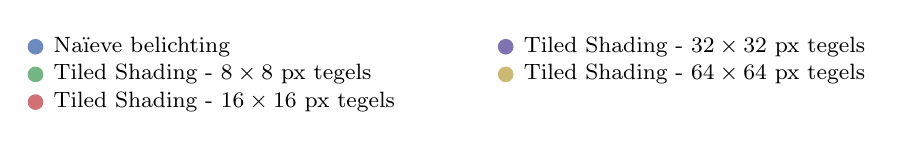
\begin{tikzpicture}
      \node (legend:naive) at (0.1\textwidth,0) [legend-point, fill={GraphBlue}, label=right:{\footnotesize Na\"ieve belichting}] {};
      \node (legend:grid) at (0.1\textwidth, -10pt) [legend-point, fill={GraphGreen}, label=right:{\footnotesize Tiled Shading - $8 \times 8$ px tegels}] {};
      \node (legend:tiled) at (0.1\textwidth, -20pt) [legend-point, fill={GraphRed}, label=right:{\footnotesize Tiled Shading - $16 \times 16$ px tegels}] {};
      
      \node (legend:tiled) at (0.5925\textwidth, -0pt) [legend-point, fill={GraphPurple}, label=right:{\footnotesize Tiled Shading - $32 \times 32$ px tegels}] {};
      \node (legend:tiled) at (0.5925\textwidth, -10pt) [legend-point, fill={GraphYellow}, label=right:{\footnotesize Tiled Shading - $64 \times 64$ px tegels}] {};
    \end{tikzpicture}
  \end{subfigure}\hfill\\
  \begin{minipage}[t]{0.5\textwidth}
  \begin{adjustbox}{minipage=\textwidth, scale=0.55}
    \begin{subfigure}[b]{1.6\textwidth}
      \centering
      \def\svgwidth{\textwidth}
      \input{./img/raw/ts-lc-lights/deferred/lights_spaceship-indoor.pdf_tex}
      \caption{Spaceship Indoor}
      \vspace{4pt}
      \label{fig:ts-lc-test-lights:indoor}
    \end{subfigure}
  \end{adjustbox} \\
  %
  \begin{adjustbox}{minipage=\textwidth, scale=0.55}
    \begin{subfigure}[b]{1.6\textwidth}
      \centering
      \def\svgwidth{\textwidth}
      \input{./img/raw/ts-lc-lights/deferred/lights_pipers-alley.pdf_tex}
      \caption{Piper's Alley}
      \vspace{4pt}
      \label{fig:ts-lc-lights:alley}
    \end{subfigure}
  \end{adjustbox} \\
  %
  \begin{adjustbox}{minipage=\textwidth, scale=0.55}
    \begin{subfigure}[b]{1.6\textwidth}
      \centering
      \def\svgwidth{\textwidth}
      \input{./img/raw/ts-lc-lights/deferred/lights_ziggurat-city.pdf_tex}
      \caption{Ziggurat City}
      \label{fig:ts-lc-lights:city}
    \end{subfigure}
  \end{adjustbox}
  \caption{\small Lichtberekeningen.}
  \label{fig:ts-lc-lights}
  \end{minipage} %
  %
  \begin{minipage}[t]{0.5\textwidth}
  \begin{adjustbox}{minipage=\textwidth, scale=0.55}
    \begin{subfigure}[b]{1.6\textwidth}
      \centering
      \def\svgwidth{\textwidth}
      \input{./img/raw/ts-lights-grid/lights_spaceship-indoor_2560.pdf_tex}
      \caption{Spaceship Indoor}
      \vspace{4pt}
      \label{fig:ts-lc-resolution:indoor}
    \end{subfigure}
  \end{adjustbox} \\
  %
  \begin{adjustbox}{minipage=\textwidth, scale=0.55}
    \begin{subfigure}[b]{1.6\textwidth}
      \centering
      \def\svgwidth{\textwidth}
      \input{./img/raw/ts-lights-grid/lights_pipers-alley_2560.pdf_tex}
      \caption{Piper's Alley}
      \vspace{4pt}
      \label{fig:ts-lights-grid:alley}
    \end{subfigure}
  \end{adjustbox} \\
  %
  \begin{adjustbox}{minipage=\textwidth, scale=0.55}
    \begin{subfigure}[b]{1.6\textwidth}
      \centering
      \def\svgwidth{\textwidth}
      \input{./img/raw/ts-lights-grid/lights_ziggurat-city_2560.pdf_tex}
      \caption{Ziggurat City}
      \label{fig:ts-lights-grid:city}
    \end{subfigure}
  \end{adjustbox}
  \caption{\small Lichtroosteropbouw. }
  \label{fig:ts-lights-grid}
  \end{minipage}
\end{figure}

